\documentclass[12pt, dvipdfmx]{beamer}
%\documentclass[8,9,10,11,12,14,17,20pt, dvips, handout]{beamer}
%%%%%%%%%%%  package  %%%%%%%%%%%
\usepackage{amssymb,amsmath,ascmac}
\usepackage{atbegshi}
\AtBeginShipoutFirst{\special{pdf:tounicode 90ms-RKSJ-UCS2}}
\usepackage{minijs}
\renewcommand{\kanjifamilydefault}{\gtdefault}
\usepackage{multirow}

\usepackage[dvipdfmx]{animate}
\usepackage{graphicx}
\usepackage{bm}

%\usepackage{tikz}
%\usepackage{xparse}
%\usetikzlibrary{shapes,arrows}
%%% define fancy arrow. \tikzfancyarrow[<option>]{<text>}. ex: \tikzfancyarrow[fill=red!5]{hoge}
%  \tikzset{arrowstyle/.style n args={2}{inner ysep=0.1ex, inner xsep=0.5em, minimum height=2em, draw=#2, fill=black!20, font=\sffamily\bfseries, single arrow, single arrow head extend=0.4em, #1,}}
%  \NewDocumentCommand{\tikzfancyarrow}{O{fill=black!20} O{none}  m}{
%    \tikz[baseline=-0.5ex]\node [arrowstyle={#1}{#2}] {#3 \mathstrut};}

%%%%%%%%%%%  theme  %%%%%%%%%%%

%%%%%
% Simple
%%%%%
%\usetheme{default}
%\usetheme{Pittsburgh}
%\usetheme{Rochester}
%\usetheme{Szeged}

%%%%%
% So So
%%%%%
%\usetheme{Singapore}
%\usetheme{CambridgeUS}
\usetheme{Copenhagen}
%\usetheme{Luebeck}
%\usetheme{Malmoe}
%\usetheme{Warsaw}

%%%%%
% No Heasder
%%%%%
%\usetheme{Madrid}
%\usetheme{Boadilla}

%%%%%
% No Footer
%%%%%
%\usetheme{Darmstadt}
%\usetheme{JuanLesPins}
%\usetheme{Montpellier}

%%%%%
% Color
%%%%%
%\usetheme{AnnArbor}

%%%%%
% Too much
%%%%%
%\usetheme{Berlin}
%\usetheme{Ilmenau}

%%%%%
% Right hand Side
%%%%%
%\usetheme{Goettingen}
%\usetheme{Marburg}

%%%%%
% Left hand Side
%%%%%
%\usetheme{PaloAlto}


%%%%%%%%%%%  inner theme  %%%%%%%%%%%
\useinnertheme{default}
%\useinnertheme{circles}
%\useinnertheme{inmargin}
%\useinnertheme{rectangles}
%\useinnertheme{rounded}


%%%%%%%%%%%  outer theme  %%%%%%%%%%%
\useoutertheme{default}
%\useoutertheme{miniframes}
%\useoutertheme{infolines}
%\useoutertheme{miniframes}
%\useoutertheme{smoothbars}
%\useoutertheme{sidebars}
%\useoutertheme{split}
%\useoutertheme{shadow}
%\useoutertheme{tree}
%\useoutertheme{smoothtree}


%%%%%%%%%%%  color theme  %%%%%%%%%%%
%\usecolortheme{structure}
%\usecolortheme{sidebartab}
%\usecolortheme{albatross}
%\usecolortheme{beetle}
%\usecolortheme{dove}
%\usecolortheme{crane}
%\usecolortheme{fly}
%\usecolortheme{seagull}
%\usecolortheme{wolverine}
%\usecolortheme{beaver}
%\usecolortheme{lily}
%\usecolortheme{orchid}
%\usecolortheme{rose}
%\usecolortheme{whale}
%\usecolortheme{seahorse}
%\usecolortheme{dolphin}


%%%%%%%%%%%  font theme  %%%%%%%%%%%
\usefonttheme{professionalfonts}
%\usefonttheme{default}
%\usefonttheme{serif}
%\usefonttheme{structurebold}
%\usefonttheme{structureserif}
%\usefonttheme{structuresmallcapsserif}


%%%%%%%%%%%  degree of transparency  %%%%%%%%%%%
%\setbeamercovered{transparent=30}

%\setbeamercolor{item}{fg=red}
\setbeamertemplate{items}[default]

%%%%%%%%%%%  numbering  %%%%%%%%%%%
%\setbeamertemplate{numbered}

\setbeamertemplate{navigation symbols}{}

\title
[DPD シミュレーションによる動的ネットワークの緩和挙動の検討]
{DPD シミュレーションによる\\動的ネットワークの緩和挙動の検討}
%{テレケリックアイオノマーを用いた超分子ネットワーク\\および\\それにより形成されるエラストマーの特性評価}
%{Characteristics Evaluation of Supra-Network formed from Telechelic Ionomers \\and Elastomer Generated Thereof}
\author[東亞合成 佐々木 近畿大学 荒井]{佐々木裕、荒井規允}
\institute[東亞合成。近畿大学]{東亞合成、近畿大学}
\date{December 9, 2016}

\begin{document}

%%%%%
% 1 P
%%%%%
\begin{frame}\frametitle{}
	\titlepage
\end{frame}

%%%%%
% 2 P
%%%%%
\section*{}
%
\begin{frame}
%[allowframebreaks]
{Outline}
	\tableofcontents
\end{frame}

\section{はじめに}

%%%%
% 3 P
%%%%%%
\subsection{背景}
%%%%%
%%%%%
\begin{frame}
%[shrink squeeze]
\frametitle{背景}

\begin{block}{「ソフトマター研究の深化」}
	\begin{itemize}
	\item
	内部自由度の高さを利用した階層的な構造設計の検討
	\item
	ソフトマターの特徴である柔らかさ+新規機能
	\item
	{\bf 力学特性の付与には\alert{ネットワーク構造}が必要}
		\begin{itemize}
		\item
		「マクロ特性」$\leftarrow$ 多段にわたる階層構造 $\rightarrow$「ミクロ構造」
		\item
		ネットワーク構造の空間的な不均一(架橋密度揺らぎ)
		\end{itemize}
	\end{itemize}
\end{block}

\begin{exampleblock}{超分子ネットワーク}<2>
	\begin{itemize}
	\item
	「繋ぎ替え可能な非共有結合」

	水素結合、疎水性相互作用、静電相互作用、等々…

	\item
	自己組織化した超分子ネットワーク
	\end{itemize}
\end{exampleblock}

\end{frame}
%%%%%

%%%%%
\begin{frame}
\frametitle{テレケリックアイオノマーの検討結果}

ESA-CF 法 (Electrostatic Self-assembly and Covalent Fixation)\\による超分子ネットワーク\\
{\scriptsize Y. Tezuka, E.J. Goethals, European Polymer Journal, 991, 1982}

\begin{columns}[T, totalwidth=\linewidth]
\column{.32\linewidth}
	{\scriptsize テレケリックアイオノマーの合成}
	\includegraphics[width=\columnwidth]{./fig/Telechelic_Anion_2.png}
	
	{\scriptsize ネットワークイメージ}
	%\vspace{3mm}
	\includegraphics[width=\columnwidth]{./fig/Network_2.pdf}
\column{.32\linewidth}<2->
	{\scriptsize 
	レオメータで、温度ジャンプにより反応性を評価
	\begin{itemize}
	\item
	疑一次反応で架橋反応を記述可能
	\item
	付加反応は反応律速
	\item
	塩構造の末端基がクラスタを形成?
	\end{itemize}
	}
	\includegraphics[width=\columnwidth]{./fig/Cure_100deg.pdf}
\column{.32\linewidth}<3>
	{\scriptsize
	形成ネットワークの力学特性
	\begin{itemize}
	\item
	古典ゴム理論で、伸長特性を記述可能
	\item
	C2 の寄与が比較的大きい
	\item
	伸び切り効果が顕著
	\end{itemize}
	}
	\includegraphics[width=\columnwidth]{./fig/SS_wMR_5_2.pdf}
\end{columns}
\end{frame}
%%%%%%%%%%%

%%%%%%%%%%%%%%%%%%%%%%%%%%%%%%%%%%%%%%%%%%%
\subsection{超分子ネットワークのモデル化}
%%%%%%%%%%%%%%%%%%%%%%%%%%%%%%%%%%%%%%%%%%%

%%%%%%%%%%%
\begin{frame}
%[shrink squeeze]
\frametitle{超分子ネットワークのモデル化}
超分子ネットワークの特徴的な構造をモデル化
	\begin{itemize}
	\item
	直鎖上の粗視化ポリマーを設定
		\begin{itemize}
		\item
		両末端に相互作用する化学種をセグメントとして設定
		\item
		セグメント間に適正な相互作用パラメタを設定\\
		$\rightarrow$引力 or 斥力
		\item
		末端セグメントが偏析したクラスタを形成
		\end{itemize}
	\item
	クラスタを介したネットワークモデルを得る
	\end{itemize}

	\begin{alertblock}{もっとも単純なモデル}<2>
		\begin{itemize}
		\item 
		トリブロックポリマー
		\item 
		BCC構造によるネットワークの形成
		\end{itemize}
	\end{alertblock}
\end{frame}
%%%%%%%%%%%

%%%%%%%%%%%%%%%%%%%%%%%%%%%%%%
\subsection{オブジェクティブ}
%%%%%%%%%%%%%%%%%%%%%%%%%%%%%%

%%%%%%%%%%%%%
\begin{frame}
\frametitle{オブジェクティブ}
	\begin{block}{テレケリックアイオノマーによるネットワークのモデル}
	トリブロックポリマーを採用し、DPDシミュレーションにより動的なネットワークの検討を行った。
	\end{block}

	\begin{exampleblock}{具体的な検討内容}<2>
		\begin{enumerate}
		\item
		クラスタ評価

		クラスタの可視化、統計的評価
		\item
		緩和時間評価
		
		偏析したクラスタを介した動的ネットワーク構造の特徴時間として応力緩和関数G(t) からの{\color{red} 終端緩和}を考え、ミクロな構造に起因した以下の二つの緩和時間と比較。
		\begin{itemize}
		\item
		{\color{blue} ポリマー鎖の末端間ベクトルの自己相関}
		\item
		{\color{blue} 末端セグメントの時空相関関数のセルフパート $G_s(\bm{r},t)$}
		\end{itemize}
		\end{enumerate}
	\end{exampleblock}
\end{frame}
%%%%%%%%%%%

%%%%%%%%%%%%%%%%%%%%%%%%%%
\section{シミュレーション}
%%%%%%%%%%%%%%%%%%%%%%%%%%
%%%%%%%%%%%%%
\begin{frame}
\LARGE{シミュレーション}
\end{frame}
%%%%%%%%%%%%

%%%%%%%%%%%%%%%%%%%%%%%%%%%%%%%%
\subsection{DPDシミュレーション}
%%%%%%%%%%%%%%%%%%%%%%%%%%%%%%%%
\begin{frame}
\frametitle{DPD法で働く三つの力と相互作用パラメタ $a_{ij}$}

	\begin{block}{粒子に働く三つの力}
	保存力 ${\bf F}_{ij}^C$、散逸力 ${\bf F}_{ij}^D$、ランダム力 ${\bf F}_{ij}^R$
	
	\begin{equation*}
	m\dfrac{{\rm d}^2 {\bf r}_i}{{\rm d} t^2} = {\bf f}_i = \sum_{j \neq i} \left( {\bf F}_{ij}^C + {\bf F}_{ij}^D + {\bf F}_{ij}^R \right)
	\end{equation*}
	\end{block}

	\begin{block}{粒子間相互作用を表すパラメタ $a_{ij}$} %<2>
	\begin{equation*}
	\mathbf{F}_{ij}^C =
	        	a_{ij} w^C (|\mathbf{r}_{ij}|) \dfrac{\mathbf{r}_{ij}}{|\mathbf{r}_{ij}|} \quad (|\mathbf{r}_{ij}| < r_c)
	\end{equation*}
	なお、$\mathbf{r}_{ij} (=\mathbf{r}_i - \mathbf{r}_j)$ は粒子間距離、$w^C (|\mathbf{r}_{ij}|)$ は粒子間距離に応じた重み関数であり、 r$_c$ はカットオフ距離を表す。
	\end{block}
\end{frame}
%%%%%

%%%%%
\begin{frame}
\frametitle{相互作用パラメタ $a_{ij}$ と $\chi$ パラメタ}

\begin{block}{相互作用パラメタ $a_{ij}$ と斥力}
	\begin{itemize}
	\item
	同種ビーズ間の $a_{ii}$ は 25(密度 $\rho =3$ の場合)。
	\item
	異種粒子間の斥力は、$a_{ij}$ の増分 $\Delta a$ で表現。
	\end{itemize}
\end{block}
\begin{exampleblock}{$\chi$ パラメタとの相関}<2>
	フローリー・ハギンス格子モデルにおける $\chi$ パラメタとは、下式の相関が報告されている。
	\begin{equation*}
	\dfrac{\chi N k_B T}{\Delta a} = (0.306 \pm 0.003) N
	\label{eq:achi}
	\end{equation*}
	なお、$N$ はセグメント数を表している。
\end{exampleblock}
\end{frame}
%%%%%%%%%%%

%%%%%%%%%%%%%
\begin{frame}
\frametitle{DPDシミュレーション}

OCTA 上の Cognac により、DPD シミュレーションを実施。

\begin{columns}[T, totalwidth=0.96\linewidth]
\column{.67\linewidth}

シミュレーション条件
	\begin{itemize}
	\item
	密度 $\rho =3$
	\item
	A1B18A1 トリブロックポリマー 1200 本(ビーズ数:24,000)
	\item
	システムサイズ $20\times20\times20$
	\item
	A, B ビーズ間に斥力を設定

	$a_{AB} = 25, 40, 50, 60, 70, 80$
	\item
	ジブロックポリマー換算では、

	$\chi N \simeq 0 \sim 170$ 程度に対応
	\end{itemize}

\column{.3\linewidth}
\includegraphics[width=\columnwidth]{./fig/polymer.png}

\includegraphics[width=\columnwidth]{./fig/all.png}
\end{columns}
\end{frame}
%%%%%%%%%%%%

%%%%%%%%%%%%%%%%%%%%%%%%%%
\subsection{評価について}
%%%%%%%%%%%%%%%%%%%%%%%%%%%

%%%%%%%%%%%%%
\begin{frame}
\frametitle{評価について}

\begin{itemize}
\item
応力緩和関数

	応力ゆらぎの自己相関関数から、Green-Kuboの表式により算出。
\item
クラスタの評価

	Stillinger クラスタとして評価。

\item
末端間ベクトルの自己相関

	末端間ベクトルの自己相関を評価し、その構造緩和を評価。

\item
時空相関関数

	時空相関関数のセルフパート $G_s(\bm{r}, t)$ を算出し、その時間変化からクラスタ内のセグメントのダイナミクスを評価
\end{itemize}

\end{frame}
%%%%%%%%%%%%

%%%%%%%%%%%%%
\begin{frame}
\frametitle{クラスタの評価}

以下に示した考え方で、クラスタの評価を行った。

\begin{columns}[c, totalwidth=\linewidth]
\column{.6\linewidth}
	\begin{itemize}
	\item
	Stillinger クラスタとして評価。
		\begin{itemize}
		\item
		判定距離 $b$ 以下の時、\\
		同一クラスタと判定
		\item
		右図の場合、\\
		4個のクラスタ:3\\
		3個のクラスタ:1\\
		2個のクラスタ:4\\
		1個のクラスタ:2
		\end{itemize}
	\item
	各タイムステップで評価
	\item
	ループ/ブリッジ判定
		\begin{itemize}
		\item
		同一クラスタに両端が\\属すかどうかで判定。	
		\end{itemize}
	\end{itemize}
\column{.36\linewidth}
\includegraphics[width=\columnwidth]{./fig/clusters.pdf}

Stillinger クラスタの考え方
\end{columns}
\end{frame}
%%%%%%%%%%%%

%%%%%%%%%%%%%
\begin{frame}
\frametitle{時空相関関数(あるいは、van Hove 関数)}
\vspace{-2mm}
\begin{columns}[T, totalwidth=\linewidth]
\column{.56\linewidth}
\begin{block}{時空相関関数 $G(\bm{r}, t)$ の定義}
\vspace{-4mm}
\scriptsize
\begin{equation*}
G(\bm{r}, t) = \dfrac{1}{N}\left\langle \sum_{i=1}^{N} \sum_{j=1}^{N} \delta[\bm{r} + \bm{r}_j(0) - \bm{r}_i(t)] \right\rangle
\end{equation*}
\normalsize
\end{block}
\vspace{-1mm}
\begin{block}{self part と distinct part}
\vspace{-4mm}
\scriptsize
\begin{align*}
	&G(\bm{r}, t) = G_s(\bm{r}, t) + G_d(\bm{r}, t) \\
	&\begin{cases}
	\text{自分自身との相関である self part:}\\
	G_s(\bm{r}, t) = \dfrac{1}{N}\left\langle \displaystyle \sum_{i=1}^{N} \delta[\bm{r} + \bm{r}_i(0) - \bm{r}_i(t)] \right\rangle \\[12pt]
	\text{異なる粒子間の相関だけの distinct part:}\\
	G_d(\bm{r}, t) = \dfrac{1}{N}\left\langle \displaystyle \sum_{i \neq j}^{N} \displaystyle \sum_{j=1}^{N} \delta[\bm{r} + \bm{r}_j(0) - \bm{r}_i(t)] \right\rangle
 	\end{cases}
\end{align*}
\normalsize
\end{block}

\column{.4\linewidth}
\includegraphics[width=\columnwidth]{./fig/G(rt).pdf}

\centering
粒子の移動のイメージ\\
$\bm{r}_i(0) \rightarrow \bm{r}_i(t)$ へと移動

\end{columns}
\end{frame}
%%%%%%%%%%%

%%%%%%%%%%
\begin{frame}
%[shrink squeeze]
%[allowframebreaks]
\frametitle{self part: $G_s(\bm{r}, t)$ によるクラスタの評価}

\begin{columns}[T, totalwidth=0.96\linewidth]
\column{.47\linewidth}

\begin{block}{$G_s(\bm{r}, t)$ の特性}
	\begin{itemize}
	\item
%	\footnotesize
	全空間で積分すれば 1\\
%	\scriptsize
%	\begin{equation*}
%	\int G_s(\bm{r}, t) {\rm d} \bm{r} = 1
%	\end{equation*}
%	\normalsize
	\item
%	\footnotesize
	$t=0$ で、デルタ関数
%	\scriptsize
%	\begin{equation*}
%	G_s(\bm{r}, 0) = \delta (\bm{r})
%	\end{equation*}
%	\normalsize
	\item
%	\footnotesize
	時間経過に伴う空間的な広がりを評価可能
	\end{itemize}
\end{block}

\begin{alertblock}{クラスタ内の評価}<3>
%\footnotesize
クラスタ空間からのセグメント脱離の評価
\end{alertblock}

\column{.47\linewidth}
\includegraphics[width=\columnwidth]{./fig/Ave_Trj.pdf}<2->

%\centering
%$G_s(\bm{r}, t)$ の例
\end{columns}
\end{frame}
%%%%%%%%%%%

%%%%%%%%%%%%%%%%%%%%%
\subsection{検討内容}
%%%%%%%%%%%%%%%%%%%%%

%%%%%%%%%%%%%
\begin{frame}
\frametitle{検討内容}
\begin{itemize}
\item
DPDシミュレーションによるネットワーク構造
	\begin{itemize}
	\item
	トリブロックポリマーのミクロ相分離構造
	\item
	末端セグメントの可視化と統計量の評価
	\end{itemize}
\item
動的ネットワークのダイナミクス特性の評価
	\begin{itemize}
	\item
	応力の自己相関からの応力緩和関数
	\item
	他の緩和時間
		\begin{itemize}
		\item
		末端間ベクトルの自己相関関数を用いたポリマー鎖の緩和
		\item
		クラスターからの脱離に基づく緩和を時空相関関数により評価
		\end{itemize}
	\end{itemize}
\item
その他の評価
\end{itemize}
\end{frame}
%%%%%%%%%%%

%%%%%%%%%%%%%%%%%%
\section{評価結果}
%%%%%%%%%%%%%%%%%%
%%%%%%%%%%%%%
\begin{frame}
\LARGE{評価結果}
\end{frame}
%%%%%%%%%%%%

%%%%%%%%%%%%%%%%%%%%%%%%%%%%%%%%%%%%%%%%%%%%%%
\subsection{DPDシミュレーションによるネットワーク構造}
%%%%%%%%%%%%%%%%%%%%%%%%%%%%%%%%%%%%%%%%%%%%%%
%%%%%%%%%%%%%
\begin{frame}
\LARGE{DPDシミュレーションによる\\ネットワーク構造}
\end{frame}
%%%%%%%%%%
%%%%%%
\begin{frame}
\frametitle{末端セグメントの偏析}

\centering
末端のセグメントだけを可視化した描像。
\vspace{3mm}

\animategraphics[height=2.in, autoplay, controls]{5}{./fig/anime_0/}{000}{020}

\end{frame}

%%%%%
\begin{frame}
\frametitle{末端セグメントの動径分布関数}
末端の A セグメントの動径分布関数 $g(r)$ を示した。
\begin{columns}[T, totalwidth=\linewidth]
\column{.45\linewidth}
	\begin{itemize}
	\item
	相互作用パラメタ $a_{AB}$ の上昇に伴い、クラスタ中の偏析が増大。
	\item
	斥力の無い $a_{AB}=25$ で、 $r\simeq1.2$ において極小値を示した。
	\item
	Stillinger クラスタの判定距離 $b$ としてこの極小値を用いた。
	\end{itemize}	
\column{.53\linewidth}
	\includegraphics[width=\columnwidth]{./fig/gr_all.pdf}

	\centering
	A セグメントの $g(r)$
\end{columns}

\end{frame}

%%%%%%
\begin{frame}
\frametitle{末端セグメントの偏析}

$b=1.2$ として、Stillinger クラスタの判定を行い、\\異なるクラスタごとに色を塗り分け。

\begin{columns}[T, totalwidth=0.96\linewidth]
\column{.47\linewidth}
	\includegraphics[width=\columnwidth]{./fig/snap_2.png}
\column{.47\linewidth}
	\includegraphics[width=\columnwidth]{./fig/snap_color.png}
\end{columns}

\end{frame}
%%%%%%%%%%%%

%%%%%%%%%%%%%
\begin{frame}
%[shrink squeeze]
%[allowframebreaks]
\frametitle{クラスタのダイナミクス}
クラスタ数、フリーセグメント、ブリッジ比の時間変化。
($a_{AB}=80$、末端セグメント数は、
$1200\times2 = 2400$
)
\begin{columns}[T, totalwidth=\linewidth]
	\column{.33\linewidth}
		\includegraphics[width=\columnwidth]{./fig/AB80/Domains.pdf}
	\column{.33\linewidth}
		\includegraphics[width=\columnwidth]{./fig/AB80/Free_Ends.pdf}
	\column{.33\linewidth}
		\includegraphics[width=\columnwidth]{./fig/AB80/B_ratio.pdf}
\end{columns}

\centering
%\small
\scalebox{0.7}
{
\begingroup
\renewcommand{\arraystretch}{1.2}
\begin{tabular}{p{2em} p{8.5em} p{8.5em} p{6em}} \hline
\hfil $a_{AB}$ \hfil	&	\hfil Num. of Clusters \hfil	&	\hfil Num. of Free Ends \hfil	&	\hfil Bridge Ratio \hfil	\\ \hline \hline
\hfil 50 \hfil			&	\hfil 107 \hfil				&	\hfil 53 \hfil				&	\hfil 0.77 \hfil				\\ 
\hfil 60 \hfil			&	\hfil 61 \hfil				&	\hfil 16 \hfil				&	\hfil 0.77 \hfil				\\ 
\hfil 70 \hfil			&	\hfil 46 \hfil				&	\hfil 5.4 \hfil				&	\hfil 0.76 \hfil				\\ 
\hfil 80 \hfil			&	\hfil 41 \hfil				&	\hfil 2.1 \hfil				&	\hfil 0.76 \hfil			\\ \hline
\end{tabular}
\endgroup
}
\end{frame}
%%%%%%%%%%%%%

%%%%%%%%%%%%%
\begin{frame}
\frametitle{クラスタの平均半径の見積もり}

クラスタ数の平均 $\overline{N_{cl}}$ から、クラスタの平均体積 $\overline{V_{cl}}$ は以下のように見積もれ、
\footnotesize
\begin{equation*}
\overline{V_{cl}} = \dfrac{1}{3}\times\dfrac{2400}{\overline{N_{cl}}}
\end{equation*}
\normalsize
さらに、球を仮定したクラスタの平均半径 $\overline{r_{cl}}$ は、
\footnotesize
\begin{equation*}
\overline{V_{cl}} = \dfrac{4\pi}{3}\overline{r_{cl}}^3
\end{equation*}
\normalsize

%結局、以下となる。

\centering
\scalebox{0.8}
{
\begingroup
\renewcommand{\arraystretch}{1.2}
\begin{tabular}{p{2em} p{4em} p{4em} p{4em}} \hline
\hfil $a_{AB}$ \hfil	&	\hfil$\overline{N_{cl}}$ \hfil	&	\hfil $\overline{V_{cl}}$ \hfil	&	\hfil $\overline{r_{cl}}$ \hfil	\\ \hline \hline
\hfil 50 \hfil			&	\hfil 107 \hfil					&	\hfil 7.5 \hfil				&	\hfil 1.2 \hfil					\\ 
\hfil 60 \hfil			&	\hfil 61 \hfil					&	\hfil 13.1 \hfil				&	\hfil 1.5 \hfil					\\ 
\hfil 70 \hfil			&	\hfil 46 \hfil					&	\hfil 17.4 \hfil				&	\hfil 1.6 \hfil					\\ 
\hfil 80 \hfil			&	\hfil 41 \hfil					&	\hfil 19.5 \hfil				&	\hfil 1.7 \hfil					\\ \hline
\end{tabular}
\endgroup
}
\end{frame}
%%%%%%%%%%%

%%%%%%%%%%%%%%%%%%%%%%%%%%%%%%%%%%%%%%
\subsection{動的ネットワークのダイナミクス特性の評価}
%%%%%%%%%%%%%%%%%%%%%%%%%%%%%%%%%%%%
\begin{frame}
\LARGE{動的ネットワークの\\ダイナミクス特性の評価}
\end{frame}
%%%%%%%%%%%%

%%%%%
\begin{frame}
%[shrink squeeze]
%[allowframebreaks]
\frametitle{応力緩和関数}

	\begin{columns}[T, totalwidth=\linewidth]
	\column{.55\linewidth}
	応力ゆらぎの自己相関関数から、以下に示した Green-Kubo 公式により、応力緩和関数 $G(t)$ を得た。
	\begin{equation*}
	G(t) = \dfrac{V}{k_B T} \langle \sigma(t) \sigma(0) \rangle
	\end{equation*}

	図中には、古典ゴム弾性理論に基づき導出された弾性率の理論値を示した。
	\begin{equation*}
	G=\nu k_B T
	\end{equation*}
	\column{.45\linewidth}
	\includegraphics[width=\columnwidth]{./fig/gt_all.pdf}

	異なる相互作用パラメタでの応力緩和関数 $G(t)$
	\end{columns}
\end{frame}


%%%%%
\begin{frame}

\frametitle{応力緩和からの終端緩和時間}
	\begin{columns}[T, totalwidth=\linewidth]
	\column{.47\linewidth}
		応力緩和関数 $G(t)$ の長時間領域を片対数プロットすることにより、
		流動に伴う終端緩和の緩和時間 $\tau_{gt}$ を見積もることができる。

		\begin{alertblock}{終端緩和時間}
		\centering
		$\tau_{gt} \simeq 3100 \quad (a_{AB} = 80)$
		\end{alertblock}
		
	\column{.47\linewidth}
		\includegraphics[width=\columnwidth]{./fig/AB80/gt_80.pdf}

	\centering
	$a_{AB} = 80$ の応力緩和関数
	\end{columns}
\end{frame}

%%%%%
\begin{frame}
%[shrink squeeze]
%[allowframebreaks]
\frametitle{末端間ベクトルの自己相関関数}

\begin{columns}[T, totalwidth=\linewidth]
\column{.47\linewidth}
ポリマー鎖の末端間ベクトルの自己相関関数を片対数プロットすることにより、ポリマー鎖の変形及び回転に伴う緩和時間を $\tau_{e2e}=7400$ と見積った。

終端緩和時間 $\tau_{gt}$ の約二倍となり、良好な相関が確認できた。
\begin{block}{緩和時間の比較}
\centering
$\tau_{e2e} \simeq {\color{red} 2 \times} \tau_{gt} (=3100)$
\end{block}

\column{.47\linewidth}
	\includegraphics[width=\columnwidth]{./fig/AB80/E2Evec_80.pdf}

\centering
	末端間ベクトルの自己相関\\関数($a_{AB} = 80$)
\end{columns}

\end{frame}
%%%%%%%%%%%

%%%%%
\begin{frame}

\frametitle{クラスタからの脱離の評価}

\begin{columns}[T, totalwidth=\linewidth]
\column{.47\linewidth}
A セグメントの時空相関関数のセルフパート $G_s(\bm{r}, t)$ を評価した。

$t=0$ において $r=0$ に立っていた $\delta$ 関数が、時間の経過に伴い、{\color{red} 空間的になまされていく過程}が確認できる。

\begin{exampleblock}{脱離の評価}
$G_s(\bm{r}, t)$ をクラスタが占めるであろう空間領域で積分し、その時間変化をモニタする。
\end{exampleblock}

\column{.47\linewidth}

	\includegraphics[width=\columnwidth]{./fig/AB80/Ave_Trj.pdf}

\centering
	$G_s(\bm{r}, t)$\\$a_{AB} = 80$
\end{columns}

\end{frame}
%%%%%%%%%%%

%%%%%
\begin{frame}
\frametitle{クラスタからの脱離の評価}

\begin{columns}[T, totalwidth=\linewidth]
\column{.47\linewidth}

クラスタ評価から求めたクラスタ半径 $\overline{r_{cl}}$ を指標と考え、各時刻において、$G_s(\bm{r}, t)$ をその空間領域で積分した。

片対数プロットにより、クラスタからのセグメント脱離の緩和時間 $\tau_{el}$ を見積もった。

\begin{alertblock}{脱離の緩和時間}
		\centering
		$\tau_{el} \simeq 4800 \quad (a_{AB} = 80)$
		\end{alertblock}
終端緩和時間 $\tau_{gt}=3100$ との相関が確認できた。
\column{.47\linewidth}

	\includegraphics[width=\columnwidth]{./fig/AB80/Cuml_data_7.pdf}

\centering
$r<\overline{r_{cl}}=1.7$ で積分\\
($a_{AB} = 80$)
\end{columns}

\end{frame}

%%%%
\begin{frame}
\frametitle{各種緩和時間の比較}

ここまでに求めた、各種緩和時間を一覧として以下に示した。

\begin{itemize}
\item
応力緩和関数から求めた終端緩和 $\tau_{gt}$
\item
ポリマー鎖の変形及び回転に伴う緩和時間 $\tau_{e2e}$
\item
クラスタからのセグメント脱離の緩和時間 $\tau_{el}$
\end{itemize}

\centering
\begin{tabular}{p{5em} p{5em} p{5em} p{5em}} \hline
\hfil $a_{AB}$ \hfil	&	\hfil $\tau_{gt}$ \hfil &	\hfil $\tau_{e2e}$ \hfil	&	\hfil $\tau_{el}$ \hfil	\\ \hline \hline
\hfil 50 \hfil			&	\hfil 54 \hfil			&	\hfil 170 \hfil				&	\hfil 120 \hfil				\\ 
\hfil 60 \hfil			&	\hfil 260 \hfil			&	\hfil 680 \hfil				&	\hfil 540 \hfil				\\ 
\hfil 70 \hfil			&	\hfil 1000 \hfil		&	\hfil 2300 \hfil			&	\hfil 1700 \hfil				\\ 
\hfil 80 \hfil			&	\hfil 3100 \hfil		&	\hfil 7400 \hfil			&	\hfil 4800 \hfil				\\ \hline
\end{tabular}


\end{frame}


%%%%%%%%%%%%%%%%%%%%%%%%%%%
\subsection{その他の事項}
%%%%%%%%%%%%%%%%%%%%%%%%%%
\begin{frame}
\LARGE{その他の事項}
\end{frame}
%%%%%%%%%%%%%%%%%%%%%%%%%%

%%%%%%
\begin{frame}
\frametitle{貯蔵及び損失弾性率}

応力緩和関数をフーリエ積分することにより、複素弾性率を得た。

	\begin{columns}[T, totalwidth=0.96\linewidth]
	\column{.47\linewidth}
		\includegraphics[width=\columnwidth]{./fig/gw_all.pdf}		
	\column{.47\linewidth}
		\includegraphics[width=\columnwidth]{./fig/AB80/gw_80.pdf}
	\end{columns}
\end{frame}
%%%%%%%%%%%

%%%%%%%%%%%%%
\begin{frame}
%[shrink squeeze]
%[allowframebreaks]
\frametitle{粘度と末端セグメントの動径分布関数}
応力緩和関数より得たゼロずり粘度と、その際の動径分布関数を以下に合わせて示した。
%\begin{equation*}
%\eta_0 = \lim_{\omega \to 0}\dfrac{G''(\omega)}{\omega}
%\end{equation*}

%\vspace{-5mm}

	\begin{columns}[T, totalwidth=0.96\linewidth]
	\column{.47\linewidth}
		\includegraphics[width=\columnwidth]{./fig/0_nendo.pdf}
	\column{.47\linewidth}
		\includegraphics[width=\columnwidth]{./fig/gr_all.pdf}
	\end{columns}
\end{frame}
%%%%%%%%%%%%%%

%%%%%%%%%%%%%
\begin{frame}
\frametitle{より強い相互作用でのラバープラトー}

\centering
		\includegraphics[width=7cm]{./fig/gt_long_all.pdf}
\end{frame}
%%%%%%%%%%%%%%


%%%%%%
\begin{frame}
\frametitle{おわりに}

動的な超分子ネットワークのモデル化を目的として、トリブロックポリマーの形成するネットワークのダイナミクスについて検討を行った。

	\begin{enumerate}
		\item
		クラスタ評価
		\begin{itemize}
			\item
			末端セグメントの形成するクラスタの可視化
			\item
			クラスタ構造の統計的な評価
		\end{itemize}
		\item
		緩和時間評価
		
		動的ネットワーク構造の特徴時間である終端緩和と、ミクロな構造に起因した以下の緩和時間との相関を確認。
		\begin{itemize}
		\item
		ポリマー鎖の末端間ベクトルの自己相関
		\item
		末端ビーズの時空相関関数のセルフパート $Gs(r,t)$
		\end{itemize}
	\end{enumerate}

\end{frame}

%%%%%
\begin{frame}
\LARGE{補足データ}
\end{frame}
%%%%%%%%%%%

%%%%%%
%\begin{frame}
%\frametitle{ゼロずり粘度}
%
%応力緩和関数は、$p$ 番目の緩和モードに対する緩和強度 $h_p$ と緩和時間 $\tau_{p,G}$ により、
%\begin{equation*}
%G(t)=\sum_{p \geq 1} h_p \exp\left( -\dfrac{t}{\tau_{p, G}} \right)
%\end{equation*}
%
%定常流動におけるゼロずり粘度は、
%\begin{align*}
%\eta_0 =\dfrac{\sigma(\infty)}{\dot{\gamma}}
%&=\int_0^{\infty}G(t') \rm{d} t' \\ \notag
%&=\left[ -\tau_{p,G} \exp \left( -\dfrac{t}{\tau_{p, G}} \right)\right]
%\end{align*}
%
%\end{frame}

%%%%%%%%%%%%%
\begin{frame}
\frametitle{クラスタのダイナミクス $a_{AB}=70$}
クラスタ数、フリーセグメント、ブリッジ比の時間変化。\\
(末端セグメント数は、$1200\times2 = 2400$
)
\begin{columns}[T, totalwidth=\linewidth]
	\column{.33\linewidth}
		\includegraphics[width=\columnwidth]{./fig/AB70/Domains.pdf}
	\column{.33\linewidth}
		\includegraphics[width=\columnwidth]{./fig/AB70/Free_Ends.pdf}
	\column{.33\linewidth}
		\includegraphics[width=\columnwidth]{./fig/AB70/B_ratio.pdf}
\end{columns}

\end{frame}
%%%%%%%%%%%%%

%%%%%%%%%%%%%
\begin{frame}
\frametitle{クラスタのダイナミクス $a_{AB}=60$}
クラスタ数、フリーセグメント、ブリッジ比の時間変化。\\
(末端セグメント数は、$1200\times2 = 2400$
)
\begin{columns}[T, totalwidth=\linewidth]
	\column{.33\linewidth}
		\includegraphics[width=\columnwidth]{./fig/AB60/Domains.pdf}
	\column{.33\linewidth}
		\includegraphics[width=\columnwidth]{./fig/AB60/Free_Ends.pdf}
	\column{.33\linewidth}
		\includegraphics[width=\columnwidth]{./fig/AB60/B_ratio.pdf}
\end{columns}

\end{frame}
%%%%%%%%%%%%%

%%%%%%%%%%%%%
\begin{frame}
\frametitle{クラスタのダイナミクス $a_{AB}=50$}
クラスタ数、フリーセグメント、ブリッジ比の時間変化。\\
(末端セグメント数は、$1200\times2 = 2400$
)
\begin{columns}[T, totalwidth=\linewidth]
	\column{.33\linewidth}
		\includegraphics[width=\columnwidth]{./fig/AB50/Domains.pdf}
	\column{.33\linewidth}
		\includegraphics[width=\columnwidth]{./fig/AB50/Free_Ends.pdf}
	\column{.33\linewidth}
		\includegraphics[width=\columnwidth]{./fig/AB50/B_ratio.pdf}
\end{columns}

\end{frame}
%%%%%%%%%%%%%

%%%%%%%%%%%%%
\begin{frame}
\frametitle{$G_s(\bm{r}, t)$ for $a_{AB}=70$}

\begin{columns}[T, totalwidth=\linewidth]
	\column{.48\linewidth}
		\includegraphics[width=\columnwidth]{./fig/AB70/Ave_Trj.pdf}
	\column{.48\linewidth}
		\includegraphics[width=\columnwidth]{./fig/AB70/Cuml_data_6.pdf}
\end{columns}

\end{frame}
%%%%%%%%%%%%%

%%%%%%%%%%%%%
\begin{frame}
\frametitle{$G_s(\bm{r}, t)$ for $a_{AB}=60$}

\begin{columns}[T, totalwidth=\linewidth]
	\column{.48\linewidth}
		\includegraphics[width=\columnwidth]{./fig/AB60/Ave_Trj.pdf}
	\column{.48\linewidth}
		\includegraphics[width=\columnwidth]{./fig/AB60/Cuml_data_5.pdf}
\end{columns}

\end{frame}
%%%%%%%%%%%%%

%%%%%%%%%%%%%
\begin{frame}
\frametitle{$G_s(\bm{r}, t)$ for $a_{AB}=50$}

\begin{columns}[T, totalwidth=\linewidth]
	\column{.48\linewidth}
 $a_{AB}=50$ としたときには、これ以上に強い相互作用の際に見られていた遷移する先のピークが見られなかった。

これは、最近接に相当するクラスタが明確には存在しないことをあらわしているのではないだろうか。

確かに動径分布関数においても、明確なピークはないようにも見える。

	\column{.48\linewidth}
		\includegraphics[width=\columnwidth]{./fig/AB50/Ave_Trj.pdf}
\end{columns}

\end{frame}
%%%%%%%%%%%%%

\end{document}
